% =============================================================================
% SECTION 4 - APPLICATIONS ET RÉSOLUTION
% =============================================================================

\section{Applications et résolution}
\label{sec:applications}

Cette section présente des exemples résolus en suivant rigoureusement l'\textbf{algorithme de résolution} présenté à la section précédente. Chaque problème est accompagné d'un schéma de situation et d'un diagramme de corps libre (DCL).

% =============================================================================
% PROBLÈMES DE STATIQUE
% =============================================================================

\subsection{Problèmes de statique (équilibre)}
\label{subsec:statique}

% -----------------------------------------------------------------------------
% STATIQUE 1 : Objet suspendu par deux câbles
% -----------------------------------------------------------------------------

\begin{exemple}[title=Statique 1 : Moteur suspendu dans une salle des machines (Maritime)]
Un moteur diesel auxiliaire de masse $m = 200$~kg est suspendu dans la salle des machines d'un navire par deux câbles. Le câble de bâbord fait un angle de 30° avec l'horizontale, celui de tribord fait un angle de 45° avec l'horizontale. Déterminer les tensions $T_1$ et $T_2$ dans chaque câble.

\tcblower

\textbf{\underline{Étape 1 — SCHÉMA et DCL}}

\begin{center}
\begin{tikzpicture}[scale=1.2]
    % Schéma de situation (gauche)
    \begin{scope}[xshift=-4cm]
        % Plafond
        \fill[pattern=north east lines] (-3,3) rectangle (2,3.3);
        \draw[thick] (-3,3) -- (2,3);
        
        % Câbles - géométrie correcte pour 30° et 45°
        % T1: angle 30° → tan(30°)=0.577, si Δy=1.5, Δx=1.5/0.577=2.6
        \draw[thick] (-2.6,3) -- (0,1.5) node[midway, above left] {$T_1$};
        % T2: angle 45° → tan(45°)=1, si Δy=1.5, Δx=1.5
        \draw[thick] (1.5,3) -- (0,1.5) node[midway, above right] {$T_2$};
        
        % Moteur
        \draw[thick, fill=gray!30] (-0.5,0.5) rectangle (0.5,1.5);
        \node at (0,1) {$m$};
        
        % Angles - lignes horizontales de référence
        \draw[dashed, gray] (-2.6,3) -- (-2.6,1.5) -- (0,1.5);
        \draw (-2.6,2.4) arc (270:330:0.6);
        \node at (-2.1,2.2) {\small $30°$};
        
        \draw[dashed, gray] (1.5,3) -- (1.5,1.5);
        \draw (1.5,2.4) arc (270:225:0.6);
        \node at (1.1,2.2) {\small $45°$};
        
        \node[below] at (-0.5,-0.2) {\textit{Schéma de situation}};
    \end{scope}
    
    % DCL (droite)
    \begin{scope}[xshift=3cm]
        % Point représentant l'objet
        \filldraw[black] (0,0) circle (3pt);
        \node[below right] at (0.15,-0.1) {moteur};
        
        % Axes
        \draw[->, thick] (0,0) -- (2,0) node[right] {$x$};
        \draw[->, thick] (0,0) -- (0,2) node[above] {$y$};
        
        % Forces
        % Poids
        \draw[->, very thick, red] (0,0) -- (0,-1.5) node[right] {$\vect{F}_g$};
        
        % Tension T1 (30° au-dessus de l'horizontale, vers la gauche)
        % cos(30°)=0.866, sin(30°)=0.5
        \draw[->, very thick, blue] (0,0) -- ({-1.5*cos(30)},{1.5*sin(30)}) node[above left] {$\vect{T}_1$};
        \draw[dashed, gray] (0,0) -- (-1.5,0);
        \draw (-0.5,0) arc (180:150:0.5);
        \node at (-0.75,0.25) {\small $30°$};
        
        % Tension T2 (45° au-dessus de l'horizontale, vers la droite)
        % cos(45°)=0.707, sin(45°)=0.707
        \draw[->, very thick, blue] (0,0) -- ({1.3*cos(45)},{1.3*sin(45)}) node[above right] {$\vect{T}_2$};
        \draw (0.5,0) arc (0:45:0.5);
        \node at (0.7,0.3) {\small $45°$};
        
        \node[below] at (0,-2.2) {\textit{Diagramme de corps libre}};
    \end{scope}
\end{tikzpicture}
\end{center}

Forces sur le moteur :
\begin{itemize}
    \item Poids : $F_g = mg = 200 \times 9{,}81 = 1962$~N (vers le bas)
    \item Tension $T_1$ : inconnue (vers le haut-gauche, à 30° de l'horizontale)
    \item Tension $T_2$ : inconnue (vers le haut-droite, à 45° de l'horizontale)
\end{itemize}

\textbf{\underline{Étape 2 — AXES}}

$x$ : horizontal, positif vers la droite

$y$ : vertical, positif vers le haut

\textbf{\underline{Étape 3 — ÉQUATIONS DE NEWTON}}

Le moteur est en équilibre : $\sum F_x = 0$ et $\sum F_y = 0$.

Décomposition des tensions :
\begin{align*}
    T_{1x} &= -T_1\cos 30° & T_{1y} &= T_1\sin 30° \\
    T_{2x} &= T_2\cos 45° & T_{2y} &= T_2\sin 45°
\end{align*}

Selon $x$ :
\begin{equation}
    -T_1\cos 30° + T_2\cos 45° = 0 \tag{1}
\end{equation}

Selon $y$ :
\begin{equation}
    T_1\sin 30° + T_2\sin 45° - mg = 0 \tag{2}
\end{equation}

\textbf{\underline{Étape 4 — ALGÈBRE}}

De l'équation (1) :
\[ T_2 = T_1 \frac{\cos 30°}{\cos 45°} = T_1 \times \frac{0{,}866}{0{,}707} = 1{,}225 \, T_1 \]

Substituons dans l'équation (2) :
\[ T_1\sin 30° + 1{,}225 \, T_1 \sin 45° = mg \]
\[ T_1 (0{,}5 + 1{,}225 \times 0{,}707) = 1962 \]
\[ T_1 \times 1{,}366 = 1962 \]

\[ \boxed{T_1 = 1436~\text{N}} \]

\[ \boxed{T_2 = 1{,}225 \times 1436 = 1760~\text{N}} \]

\textbf{Vérification :} $T_2 > T_1$ car le câble de droite est plus vertical (45° > 30°), il supporte donc une plus grande partie du poids. 

Vérifions $\sum F_y$ : $1436 \times 0{,}5 + 1760 \times 0{,}707 = 718 + 1244 = 1962$~N $\checkmark$

\end{exemple}

\begin{pratiqueautonome}[title=Pratique autonome 2.3 — Feu de navigation suspendu (Maritime)]
Un feu de navigation de masse $m = 12$~kg est suspendu entre deux mâts d'un navire par deux câbles. Le câble de bâbord fait un angle de 40° avec l'horizontale, celui de tribord fait un angle de 55° avec l'horizontale.

\begin{enumerate}
    \item Dessinez le DCL du feu de navigation.
    \item Calculez les tensions $T_1$ et $T_2$ dans chaque câble.
\end{enumerate}

\vspace{3cm}

\tcblower
\textit{Réponses :} $T_1 = 85{,}6$~N ; $T_2 = 79{,}8$~N
\end{pratiqueautonome}

% -----------------------------------------------------------------------------
% STATIQUE 2 : Bloc sur plan incliné à l'équilibre
% -----------------------------------------------------------------------------

\begin{exemple}[title=Statique 2 : Bloc sur plan incliné à l'équilibre]
Un bloc de masse $m = 15$~kg est posé sur un plan incliné à $\theta = 25°$ par rapport à l'horizontale. Le bloc reste immobile. Le coefficient de frottement statique entre le bloc et le plan est $\mu_s = 0{,}5$.

a) Calculer la force de frottement statique qui maintient le bloc en équilibre.

b) Quel est l'angle maximal avant que le bloc ne commence à glisser?

\tcblower

\textbf{\underline{Étape 1 — SCHÉMA et DCL}}

\begin{center}
\begin{tikzpicture}[scale=1.0]
    % Schéma de situation (gauche)
    \begin{scope}[xshift=-4.5cm]
        % Plan incliné
        \draw[thick, fill=gray!20] (0,0) -- (4,0) -- (4,1.87) -- cycle;
        \draw[thick] (0,0) -- (4,1.87);
        
        % Bloc
        \begin{scope}[rotate=25, shift={(1.5,0)}]
            \draw[thick, fill=blue!20] (0,0) rectangle (1,0.7);
            \node at (0.5,0.35) {$m$};
        \end{scope}
        
        % Angle
        \draw (1,0) arc (0:25:1) node[right, pos=0.5] {$\theta$};
        
        % Sol
        \fill[pattern=north east lines] (-0.3,-0.3) rectangle (4.3,0);
        
        \node[below] at (2,-0.8) {\textit{Schéma de situation}};
    \end{scope}
    
    % DCL (droite) - repère incliné: x // pente (+ vers bas), y ⊥ pente (+ vers ext.)
    \begin{scope}[xshift=3cm]
        % Point représentant le bloc
        \filldraw[black] (0,0) circle (3pt);
        
        % Axes inclinés (x vers le bas de la pente = vers la droite ici)
        \draw[->, thick] (0,0) -- (2.5,0) node[right] {$x$};
        \draw[->, thick] (0,0) -- (0,2) node[above] {$y$};
        \node[below right] at (2.5,-0.3) {\small (// pente, $+$ vers bas)};
        \node[left] at (-0.3,2) {\small ($\perp$ pente)};
        
        % Ligne de la pente (pour référence)
        \draw[gray, dashed] (-0.5,0) -- (2.5,0);
        
        % Forces
        % Poids VERTICAL vers le bas = dans repère incliné: (+x, -y)
        % θ=25°: Fg fait angle θ avec l'axe -y
        % Fg_x = mg·sin(25°) ≈ 0.42·mg (positif, vers bas pente)
        % Fg_y = -mg·cos(25°) ≈ -0.91·mg (négatif, vers la pente)
        \draw[->, very thick, red] (0,0) -- ({1.8*sin(25)},{-1.8*cos(25)}) node[below right] {$\vect{F}_g$};
        
        % Composantes du poids (en pointillés)
        \draw[->, thick, red, dashed] (0,0) -- ({1.8*sin(25)},0) node[above] {\small $mg\sin\theta$};
        \draw[->, thick, red, dashed] (0,0) -- (0,{-1.8*cos(25)}) node[right] {\small $mg\cos\theta$};
        
        % Normale (perpendiculaire au plan, vers l'extérieur = +y)
        \draw[->, very thick, green!60!black] (0,0) -- (0,{1.8*cos(25)}) node[above] {$\vect{N}$};
        
        % Frottement (parallèle au plan, vers le HAUT de la pente = -x)
        \draw[->, very thick, orange] (0,0) -- ({-1.8*sin(25)},0) node[above left] {$\vect{f}_s$};
        
        % Angle du poids avec l'axe -y
        \draw[red] ({0.4*sin(25)},{-0.5}) arc (250:270:0.5);
        \node[red] at (0.5,-0.7) {\small $\theta$};
        
        \node[below] at (0,-2.2) {\textit{Diagramme de corps libre}};
    \end{scope}
\end{tikzpicture}
\end{center}

Forces sur le bloc :
\begin{itemize}
    \item Poids : $F_g = mg$ (vertical vers le bas)
    \item Normale : $N$ (perpendiculaire au plan, vers l'extérieur)
    \item Frottement statique : $f_s$ (parallèle au plan, vers le haut de la pente)
\end{itemize}

\textbf{\underline{Étape 2 — AXES}}

$x$ : parallèle à la pente, positif vers le bas

$y$ : perpendiculaire à la pente, positif vers l'extérieur

Avec ce choix, si le bloc bouge, son accélération sera selon $x$ uniquement.

\textbf{\underline{Étape 3 — ÉQUATIONS DE NEWTON}}

Décomposition du poids :
\begin{align*}
    F_{g,x} &= mg\sin\theta \\
    F_{g,y} &= -mg\cos\theta
\end{align*}

Équilibre selon $y$ ($a_y = 0$) :
\begin{equation}
    N - mg\cos\theta = 0 \implies N = mg\cos\theta \tag{1}
\end{equation}

Équilibre selon $x$ ($a_x = 0$) :
\begin{equation}
    mg\sin\theta - f_s = 0 \implies f_s = mg\sin\theta \tag{2}
\end{equation}

\textbf{\underline{Étape 4 — ALGÈBRE}}

\textbf{a) Force de frottement :}
\[ f_s = mg\sin\theta = 15 \times 9{,}81 \times \sin 25° = 147{,}2 \times 0{,}423 \]
\[ \boxed{f_s = 62{,}2~\text{N}} \]

Vérifions que le bloc peut rester en équilibre. La normale vaut :
\[ N = mg\cos\theta = 15 \times 9{,}81 \times \cos 25° = 133{,}4~\text{N} \]

Le frottement statique maximal est :
\[ f_{s,\max} = \mu_s N = 0{,}5 \times 133{,}4 = 66{,}7~\text{N} \]

Comme $f_s = 62{,}2~\text{N} < f_{s,\max} = 66{,}7~\text{N}$, le bloc reste bien en équilibre. $\checkmark$

\textbf{b) Angle maximal :}

À la limite du glissement, $f_s = f_{s,\max} = \mu_s N$. En combinant avec les équations d'équilibre :
\[ mg\sin\theta_{\max} = \mu_s \cdot mg\cos\theta_{\max} \]
\[ \tan\theta_{\max} = \mu_s \]
\[ \theta_{\max} = \arctan(\mu_s) = \arctan(0{,}5) \]
\[ \boxed{\theta_{\max} = 26{,}6°} \]

Au-delà de cet angle, le bloc commencera à glisser.

\end{exemple}

\begin{pratiqueautonome}[title=Pratique autonome 2.4 — Caisse sur rampe de navire (Maritime)]
Une caisse de marchandise de 80~kg est posée sur une rampe de chargement d'un cargo, inclinée à 22°. Le coefficient de frottement statique est $\mu_s = 0{,}45$.

\begin{enumerate}
    \item La caisse reste-t-elle en équilibre? (Calculez la force de frottement nécessaire vs disponible)
    \item Si oui, quelle force horizontale minimale faudrait-il appliquer pour la faire glisser vers le haut?
\end{enumerate}

\vspace{3.5cm}

\tcblower
\textit{Réponses :} 1) Oui, $f_{\text{néc}} = 294$~N $<$ $f_{\text{max}} = 327$~N \quad 2) $F = 652$~N
\end{pratiqueautonome}

% -----------------------------------------------------------------------------
% STATIQUE 3 : Système avec poulie
% -----------------------------------------------------------------------------

\begin{exemple}[title=Statique 3 : Système avec poulie simple]
Un bloc A de masse $m_A = 5$~kg est posé sur une table horizontale. Il est relié par une corde passant par une poulie sans frottement à un bloc B de masse $m_B$ suspendu dans le vide. Le coefficient de frottement statique entre le bloc A et la table est $\mu_s = 0{,}4$.

Quelle est la masse maximale $m_B$ pour que le système reste en équilibre?

\tcblower

\textbf{\underline{Étape 1 — SCHÉMA et DCL}}

\begin{center}
\begin{tikzpicture}[scale=0.95]
    % Schéma de situation (gauche)
    \begin{scope}[xshift=-4.5cm]
        % Table
        \fill[pattern=north east lines] (-0.5,-0.3) rectangle (3,0);
        \draw[thick] (-0.5,0) -- (3,0);
        
        % Bloc A
        \draw[thick, fill=blue!20] (0.5,0) rectangle (1.8,0.8);
        \node at (1.15,0.4) {$A$};
        
        % Poulie
        \draw[thick] (3,0.5) circle (0.4);
        \filldraw[black] (3,0.5) circle (2pt);
        \draw[thick] (2.6,0.5) -- (2.6,1.2) -- (3.4,1.2) -- (3.4,0.5);
        \fill[pattern=north east lines] (2.6,1.2) rectangle (3.4,1.5);
        
        % Corde
        \draw[thick] (1.8,0.4) -- (2.6,0.4) arc (180:270:0.1) -- (2.7,0.1);
        \draw[thick] (3,0.1) -- (3,-1.5);
        
        % Bloc B
        \draw[thick, fill=red!20] (2.5,-1.5) rectangle (3.5,-2.3);
        \node at (3,-1.9) {$B$};
        
        \node[below] at (1.5,-2.8) {\textit{Schéma de situation}};
    \end{scope}
    
    % DCL bloc A (milieu)
    \begin{scope}[xshift=0.5cm, yshift=0.5cm]
        \node[above] at (0,1.8) {\textbf{Bloc A}};
        
        % Point
        \filldraw[black] (0,0) circle (3pt);
        
        % Axes
        \draw[->, thick] (0,0) -- (1.8,0) node[right] {$x$};
        \draw[->, thick] (0,0) -- (0,1.5) node[above] {$y$};
        
        % Forces
        \draw[->, very thick, red] (0,0) -- (0,-1.2) node[right] {$m_A g$};
        \draw[->, very thick, green!60!black] (0,0) -- (0,1.2) node[left] {$N$};
        \draw[->, very thick, blue] (0,0) -- (1.2,0) node[above] {$T$};
        \draw[->, very thick, orange] (0,0) -- (-0.8,0) node[above] {$f_s$};
        
        \node[below] at (0,-1.8) {\textit{DCL bloc A}};
    \end{scope}
    
    % DCL bloc B (droite)
    \begin{scope}[xshift=4.5cm, yshift=0.5cm]
        \node[above] at (0,1.8) {\textbf{Bloc B}};
        
        % Point
        \filldraw[black] (0,0) circle (3pt);
        
        % Axes
        \draw[->, thick] (0,0) -- (1.5,0) node[right] {$x$};
        \draw[->, thick] (0,0) -- (0,1.5) node[above] {$y$};
        
        % Forces
        \draw[->, very thick, red] (0,0) -- (0,-1.2) node[right] {$m_B g$};
        \draw[->, very thick, blue] (0,0) -- (0,0.8) node[left] {$T$};
        
        \node[below] at (0,-1.8) {\textit{DCL bloc B}};
    \end{scope}
\end{tikzpicture}
\end{center}

\textbf{Bloc A :} Poids $m_A g$ (bas), Normale $N$ (haut), Tension $T$ (droite), Frottement $f_s$ (gauche)

\textbf{Bloc B :} Poids $m_B g$ (bas), Tension $T$ (haut)

\textit{Note :} La tension est la même des deux côtés car la poulie est sans frottement et la corde est de masse négligeable.

\textbf{\underline{Étape 2 — AXES}}

Pour les deux blocs : $x$ horizontal (positif vers la droite), $y$ vertical (positif vers le haut).

\textbf{\underline{Étape 3 — ÉQUATIONS DE NEWTON}}

\textbf{Bloc A} (équilibre) :

Selon $y$ : 
\begin{equation}
    N - m_A g = 0 \implies N = m_A g \tag{A-y}
\end{equation}

Selon $x$ : 
\begin{equation}
    T - f_s = 0 \implies T = f_s \tag{A-x}
\end{equation}

\textbf{Bloc B} (équilibre) :

Selon $y$ : 
\begin{equation}
    T - m_B g = 0 \implies T = m_B g \tag{B-y}
\end{equation}

\textbf{\underline{Étape 4 — ALGÈBRE}}

Des équations (A-x) et (B-y) : $f_s = m_B g$

Pour que le système reste en équilibre, le frottement doit pouvoir retenir le bloc A :
\[ f_s \leq \mu_s N = \mu_s m_A g \]

Donc :
\[ m_B g \leq \mu_s m_A g \]
\[ m_B \leq \mu_s m_A \]

La masse maximale de B est :
\[ m_{B,\max} = \mu_s m_A = 0{,}4 \times 5 = \boxed{2{,}0~\text{kg}} \]

\textbf{Vérification :} Si $m_B = 2$~kg, alors $T = m_B g = 19{,}6$~N et $f_s = 19{,}6$~N.

Le frottement maximal disponible est $f_{s,\max} = \mu_s m_A g = 0{,}4 \times 5 \times 9{,}81 = 19{,}6$~N.

On est exactement à la limite : $f_s = f_{s,\max}$ $\checkmark$

\end{exemple}

\begin{pratiqueautonome}[title=Pratique autonome 2.5 — Système de déchargement portuaire (Maritime)]
Sur un quai, une caisse A de masse $m_A = 80$~kg est posée sur une rampe inclinée à 30° (sans frottement). Elle est reliée par un câble passant par une poulie à un contrepoids B suspendu au-dessus de l'eau.

\begin{enumerate}
    \item Dessinez les DCL de la caisse A et du contrepoids B.
    \item Quelle doit être la masse $m_B$ du contrepoids pour que le système soit en équilibre?
\end{enumerate}

\vspace{4cm}

\tcblower
\textit{Réponse :} $m_B = m_A \sin 30° = 40$~kg
\end{pratiqueautonome}

% =============================================================================
% PROBLÈMES DE DYNAMIQUE
% =============================================================================

\subsection{Problèmes de dynamique}
\label{subsec:dynamique}

% -----------------------------------------------------------------------------
% DYNAMIQUE 1 : Bateau moteur (1D)
% -----------------------------------------------------------------------------

\begin{exemple}[title=Dynamique 1 : Accélération d'un navire]
Le traversier F.A. Gauthier a une masse de $m = 5000$ tonnes métriques. Ses moteurs peuvent fournir une poussée maximale de $F_p = 250$~kN. En négligeant la résistance de l'eau :

a) Quelle est l'accélération maximale du navire?

b) Combien de temps lui faut-il pour atteindre 10 nœuds (5{,}14~m/s) en partant du repos?

\tcblower

\textbf{\underline{Étape 1 — SCHÉMA et DCL}}

\begin{center}
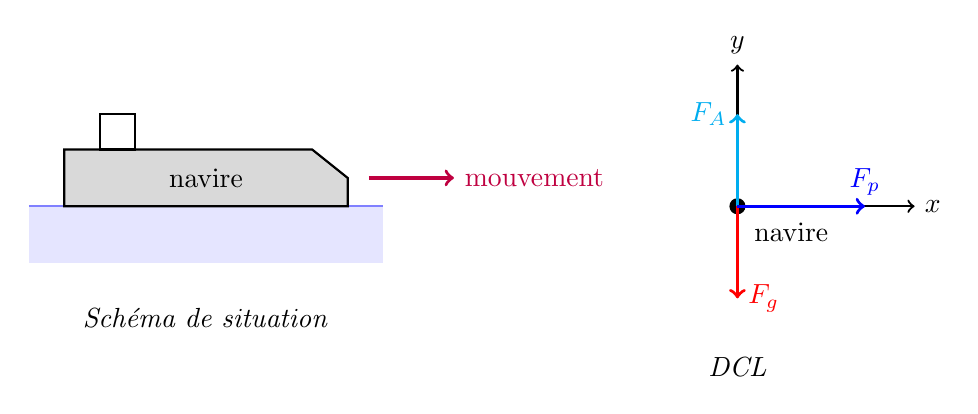
\begin{tikzpicture}[scale=0.9]
    % Schéma de situation (gauche)
    \begin{scope}[xshift=-4.5cm]
        % Eau
        \fill[blue!10] (-2,-0.8) rectangle (3,0);
        \draw[blue!50, thick] (-2,0) -- (3,0);
        
        % Navire (forme simplifiée)
        \draw[thick, fill=gray!30] 
            (-1.5,0) -- (-1.5,0.8) -- (2,0.8) -- (2.5,0.4) -- (2.5,0) -- cycle;
        \draw[thick, fill=white] (-1,0.8) rectangle (-0.5,1.3);
        \node at (0.5,0.4) {navire};
        
        % Flèche mouvement
        \draw[->, very thick, purple] (2.8,0.4) -- (4,0.4) node[right] {mouvement};
        
        \node[below] at (0.5,-1.3) {\textit{Schéma de situation}};
    \end{scope}
    
    % DCL (droite)
    \begin{scope}[xshift=3.5cm]
        % Point
        \filldraw[black] (0,0) circle (3pt);
        \node[below right] at (0.1,-0.1) {navire};
        
        % Axes
        \draw[->, thick] (0,0) -- (2.5,0) node[right] {$x$};
        \draw[->, thick] (0,0) -- (0,2) node[above] {$y$};
        
        % Forces
        \draw[->, very thick, red] (0,0) -- (0,-1.3) node[right] {$\vect{F}_g$};
        \draw[->, very thick, cyan] (0,0) -- (0,1.3) node[left] {$\vect{F}_A$};
        \draw[->, very thick, blue] (0,0) -- (1.8,0) node[above] {$\vect{F}_p$};
        
        \node[below] at (0,-2) {\textit{DCL}};
    \end{scope}
\end{tikzpicture}
\end{center}

Forces sur le navire :
\begin{itemize}
    \item Poids : $F_g = mg$ (vers le bas)
    \item Poussée d'Archimède : $F_A$ (vers le haut, compense le poids)
    \item Force de propulsion : $F_p = 250$~kN (horizontale, vers l'avant)
\end{itemize}

\textbf{\underline{Étape 2 — AXES}}

$x$ : horizontal, positif vers l'avant (sens du mouvement)

$y$ : vertical, positif vers le haut

\textbf{\underline{Étape 3 — ÉQUATIONS DE NEWTON}}

Selon $y$ (le navire ne coule pas et ne s'envole pas, donc $a_y = 0$) :
\begin{equation}
    F_A - F_g = 0 \implies F_A = mg \tag{équilibre vertical}
\end{equation}

Selon $x$ :
\begin{equation}
    F_p = ma_x \tag{dynamique horizontale}
\end{equation}

\textbf{\underline{Étape 4 — ALGÈBRE}}

\textbf{a) Accélération :}
\[ a_x = \frac{F_p}{m} = \frac{250\,000~\text{N}}{5\,000\,000~\text{kg}} = \boxed{0{,}05~\text{m/s}^2} \]

\textbf{b) Temps pour atteindre $v = 5{,}14$~m/s :}

En MRUA avec $v_0 = 0$ : $v = v_0 + at$
\[ t = \frac{v - v_0}{a} = \frac{5{,}14 - 0}{0{,}05} = \boxed{103~\text{s} \approx 1{,}7~\text{min}} \]

\textbf{Vérification :} L'accélération est très faible (0,05~m/s²) comparée à une voiture ($\sim$3~m/s²), ce qui est cohérent avec la masse énorme du navire. Le temps de 1,7 min pour atteindre 10 nœuds est réaliste pour un traversier.

\end{exemple}

\begin{pratiqueautonome}[title=Pratique autonome 2.6 — Remorqueur en action]
Un remorqueur tire un cargo de 12\,000 tonnes avec une force de 180~kN. La résistance de l'eau exerce une force opposée de $R = 0{,}8v^2$ (avec $R$ en kN et $v$ en m/s).

\begin{enumerate}
    \item Quelle est l'accélération initiale du cargo (partant du repos)?
    \item Quelle sera la vitesse maximale (de croisière) du cargo?
\end{enumerate}

\vspace{3cm}

\tcblower
\textit{Réponses :} 1) $a = 0{,}015$~m/s² \quad 2) $v_{\max} = 15$~m/s $= 29{,}2$~nœuds
\end{pratiqueautonome}

% -----------------------------------------------------------------------------
% DYNAMIQUE 2 : Remorqueurs (2D)
% -----------------------------------------------------------------------------

\begin{exemple}[title=Dynamique 2 : Remorqueurs poussant un navire]
Deux remorqueurs poussent un navire de masse $m = 8000$ tonnes pour le manœuvrer dans un port. Le remorqueur 1 exerce une force $F_1 = 60$~kN vers le nord. Le remorqueur 2 exerce une force $F_2 = 80$~kN vers l'est. En négligeant la résistance de l'eau, calculer l'accélération du navire (module et direction).

\tcblower

\textbf{\underline{Étape 1 — SCHÉMA et DCL}}

\begin{center}
\begin{tikzpicture}[scale=0.85]
    % Schéma de situation (gauche) - vue de dessus
    \begin{scope}[xshift=-4.5cm]
        \node[above] at (0,2.5) {\small Vue de dessus};
        
        % Navire (rectangle)
        \draw[thick, fill=gray!30, rotate=15] (-1.2,-0.6) rectangle (1.2,0.6);
        
        % Remorqueur 1 (sud du navire)
        \draw[thick, fill=orange!50] (-0.8,-1.5) rectangle (-0.3,-1);
        \node[below] at (-0.55,-1.5) {\small R1};
        \draw[->, very thick, blue] (-0.55,-1) -- (-0.55,0.5) node[left] {$\vect{F}_1$};
        
        % Remorqueur 2 (ouest du navire)
        \draw[thick, fill=orange!50] (-2,-0.3) rectangle (-1.5,0.3);
        \node[left] at (-2,0) {\small R2};
        \draw[->, very thick, red] (-1.5,0) -- (0.5,0) node[above] {$\vect{F}_2$};
        
        % Boussole
        \draw[->, thick] (2,1.5) -- (2,2.3) node[above] {N};
        \draw[->, thick] (2,1.5) -- (2.8,1.5) node[right] {E};
        
        \node[below] at (0,-2.2) {\textit{Schéma de situation}};
    \end{scope}
    
    % DCL (droite) - vue de dessus
    \begin{scope}[xshift=3.5cm]
        % Point
        \filldraw[black] (0,0) circle (3pt);
        \node[below left] at (-0.1,-0.1) {navire};
        
        % Axes
        \draw[->, thick] (0,0) -- (2.5,0) node[right] {$x$ (E)};
        \draw[->, thick] (0,0) -- (0,2.3) node[above] {$y$ (N)};
        
        % Forces
        \draw[->, very thick, blue] (0,0) -- (0,1.5) node[left] {$\vect{F}_1$};
        \draw[->, very thick, red] (0,0) -- (2,0) node[below] {$\vect{F}_2$};
        
        % Résultante
        \draw[->, ultra thick, purple] (0,0) -- (2,1.5) node[above right] {$\vect{F}_{\text{rés}}$};
        \draw[dashed, gray] (2,0) -- (2,1.5) -- (0,1.5);
        
        % Angle
        \draw[purple] (0.6,0) arc (0:36.87:0.6) node[right, pos=0.6] {$\theta$};
        
        \node[below] at (0.8,-1) {\textit{DCL (vue de dessus)}};
    \end{scope}
\end{tikzpicture}
\end{center}

Forces sur le navire (vue de dessus, on ignore les forces verticales qui s'annulent) :
\begin{itemize}
    \item Force du remorqueur 1 : $F_1 = 60$~kN vers le nord
    \item Force du remorqueur 2 : $F_2 = 80$~kN vers l'est
\end{itemize}

\textbf{\underline{Étape 2 — AXES}}

$x$ : vers l'est

$y$ : vers le nord

\textbf{\underline{Étape 3 — ÉQUATIONS DE NEWTON}}

Selon $x$ :
\begin{equation}
    F_2 = ma_x \implies a_x = \frac{F_2}{m} \tag{1}
\end{equation}

Selon $y$ :
\begin{equation}
    F_1 = ma_y \implies a_y = \frac{F_1}{m} \tag{2}
\end{equation}

\textbf{\underline{Étape 4 — ALGÈBRE}}

Composantes de l'accélération :
\[ a_x = \frac{80\,000}{8\,000\,000} = 0{,}01~\text{m/s}^2 \]
\[ a_y = \frac{60\,000}{8\,000\,000} = 0{,}0075~\text{m/s}^2 \]

Module de l'accélération :
\[ a = \sqrt{a_x^2 + a_y^2} = \sqrt{0{,}01^2 + 0{,}0075^2} = \sqrt{0{,}000156} = \boxed{0{,}0125~\text{m/s}^2} \]

Direction (angle par rapport à l'est) :
\[ \theta = \arctan\left(\frac{a_y}{a_x}\right) = \arctan\left(\frac{0{,}0075}{0{,}01}\right) = \arctan(0{,}75) = \boxed{36{,}9°~\text{nord de l'est}} \]

\textbf{Vérification :} On peut aussi calculer via la force résultante :
\[ F_{\text{rés}} = \sqrt{60^2 + 80^2} = \sqrt{3600 + 6400} = 100~\text{kN} \]
\[ a = \frac{F_{\text{rés}}}{m} = \frac{100\,000}{8\,000\,000} = 0{,}0125~\text{m/s}^2 \quad \checkmark \]

\end{exemple}

\begin{pratiqueautonome}[title=Pratique autonome 2.7 — Positionnement de bouée (Maritime)]
Trois câbles tirent sur un anneau au sol pour positionner une bouée de navigation. Le câble 1 exerce une force de 500~N vers le nord. Le câble 2 exerce une force de 400~N à 60° est du nord. Le câble 3 exerce une force de 300~N à 45° ouest du sud.

Déterminez la force résultante (module et direction) agissant sur l'anneau.

\vspace{4cm}

\tcblower
\textit{Réponse :} $F_{\text{rés}} = 538$~N à $30{,}5°$ est du nord
\end{pratiqueautonome}

% -----------------------------------------------------------------------------
% DYNAMIQUE 3 : Skieur sur plan incliné
% -----------------------------------------------------------------------------

\begin{exemple}[title=Dynamique 3 : Skieur sur une pente]
Un skieur de masse $m = 75$~kg descend une pente inclinée à $\theta = 20°$ par rapport à l'horizontale. Le coefficient de frottement cinétique entre les skis et la neige est $\mu_c = 0{,}08$. Calculer l'accélération du skieur.

\tcblower

\textbf{\underline{Étape 1 — SCHÉMA et DCL}}

\begin{center}
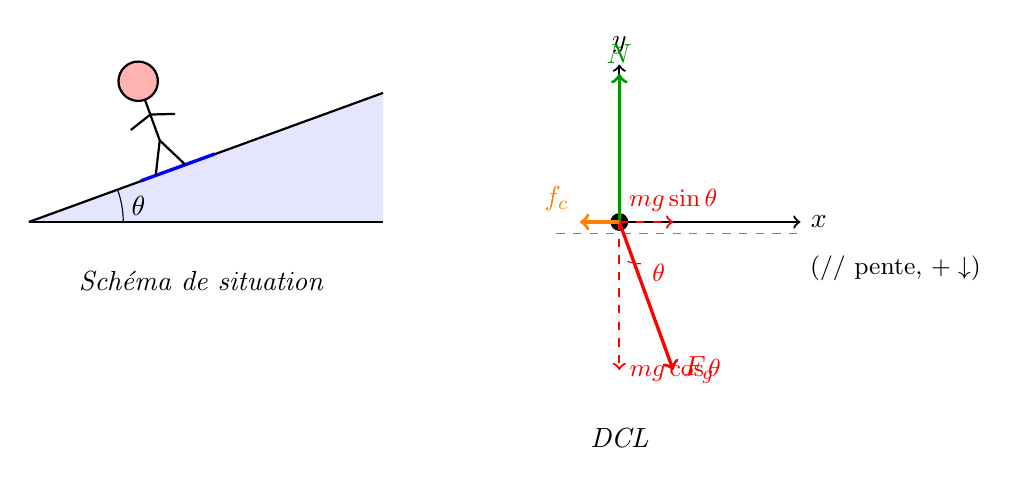
\begin{tikzpicture}[scale=1.0]
    % Schéma de situation (gauche)
    \begin{scope}[xshift=-4.5cm]
        % Pente
        \fill[white!90!blue] (0,0) -- (4.5,0) -- (4.5,1.64) -- cycle;
        \draw[thick] (0,0) -- (4.5,1.64);
        \draw[thick] (0,0) -- (4.5,0);
        
        % Skieur (bonhomme simplifié) — placé sur la pente
        % Point d'appui choisi sur la pente : (x,y) = (1.8, 0.66) car y ≈ (1.64/4.5)·x
        \begin{scope}[shift={(1.8,0.66)}, rotate=20]
            % Skis (sur la pente)
            \draw[very thick, blue] (-0.4,0) -- (0.6,0);

            % Jambes
            \draw[thick] (0,0.4) -- (-0.2,0);
            \draw[thick] (0,0.4) -- (0.2,0);

            % Tronc
            \draw[thick] (0,0.4) -- (0,0.95);

            % Bras
            \draw[thick] (0,0.75) -- (-0.3,0.65);
            \draw[thick] (0,0.75) -- (0.3,0.65);

            % Tête
            \draw[thick, fill=red!30] (0,1.2) circle (0.25);
        \end{scope}
        
        % Angle
        \draw (1.2,0) arc (0:20:1.2) node[right, pos=0.5] {$\theta$};
        

        \node[below] at (2.2,-0.5) {\textit{Schéma de situation}};
    \end{scope}
    
    % DCL (droite) - repère incliné avec x vers le bas de la pente
    \begin{scope}[xshift=3cm]
        % Point
        \filldraw[black] (0,0) circle (3pt);
        
        % Axes inclinés
        \draw[->, thick] (0,0) -- (2.3,0) node[right] {$x$};
        \draw[->, thick] (0,0) -- (0,2) node[above] {$y$};
        \node[below right] at (2.3,-0.3) {\small (// pente, $+\downarrow$)};
        
        % Surface suggérée
        \draw[gray, dashed] (-0.8,-0.15) -- (2.3,-0.15);
        
        % Poids VERTICAL: dans le repère incliné, il a des composantes (+x, -y)
        % θ=20°: sin(20°)=0.342, cos(20°)=0.940
        % Fg = (mg·sin20°, -mg·cos20°) en repère incliné
        \draw[->, very thick, red] (0,0) -- ({2*sin(20)},{-2*cos(20)}) node[right] {$\vect{F}_g$};
        
        % Composantes du poids (en pointillés)
        \draw[->, thick, red, dashed] (0,0) -- ({2*sin(20)},0) node[above] {\small $mg\sin\theta$};
        \draw[->, thick, red, dashed] (0,0) -- (0,{-2*cos(20)}) node[right] {\small $mg\cos\theta$};
        
        % Normale
        \draw[->, very thick, green!60!black] (0,0) -- (0,{2*cos(20)}) node[above] {$\vect{N}$};
        
        % Frottement (vers le haut de la pente = -x)
        \draw[->, very thick, orange] (0,0) -- (-0.5,0) node[above left] {$\vect{f}_c$};
        
        % Angle du poids avec l'axe -y
        \draw[red] ({0.3*sin(20)},{-0.5}) arc (250:270:0.5);
        \node[red] at (0.5,-0.65) {\small $\theta$};
        
        \node[below] at (0,-2.5) {\textit{DCL}};
    \end{scope}
\end{tikzpicture}
\end{center}

Forces sur le skieur :
\begin{itemize}
    \item Poids : $F_g = mg$ (vertical vers le bas)
    \item Normale : $N$ (perpendiculaire à la pente)
    \item Frottement cinétique : $f_c = \mu_c N$ (parallèle à la pente, vers le haut car il s'oppose au mouvement)
\end{itemize}

\textbf{\underline{Étape 2 — AXES}}

$x$ : parallèle à la pente, positif vers le bas de la pente

$y$ : perpendiculaire à la pente, positif vers l'extérieur

\textbf{\underline{Étape 3 — ÉQUATIONS DE NEWTON}}

Décomposition du poids :
\[ F_{g,x} = mg\sin\theta \qquad F_{g,y} = -mg\cos\theta \]

Selon $y$ (pas de mouvement perpendiculaire à la pente, $a_y = 0$) :
\begin{equation}
    N - mg\cos\theta = 0 \implies N = mg\cos\theta \tag{1}
\end{equation}

Selon $x$ (le skieur accélère vers le bas) :
\begin{equation}
    mg\sin\theta - f_c = ma_x \tag{2}
\end{equation}

Avec $f_c = \mu_c N = \mu_c mg\cos\theta$ :
\[ mg\sin\theta - \mu_c mg\cos\theta = ma_x \]
\[ a_x = g(\sin\theta - \mu_c\cos\theta) \]

\textbf{\underline{Étape 4 — ALGÈBRE}}

\[ a_x = 9{,}81 \times (\sin 20° - 0{,}08 \times \cos 20°) \]
\[ a_x = 9{,}81 \times (0{,}342 - 0{,}08 \times 0{,}940) \]
\[ a_x = 9{,}81 \times (0{,}342 - 0{,}075) \]
\[ a_x = 9{,}81 \times 0{,}267 \]
\[ \boxed{a_x = 2{,}62~\text{m/s}^2} \]

\textbf{Vérification :} 
\begin{itemize}
    \item Sans frottement ($\mu_c = 0$), on aurait $a = g\sin 20° = 3{,}35$~m/s². Le frottement réduit bien l'accélération.
    \item L'accélération est positive, donc le skieur accélère bien vers le bas.
    \item La formule $a = g(\sin\theta - \mu_c\cos\theta)$ ne dépend pas de la masse! Tous les skieurs accélèrent de la même façon sur cette pente (en négligeant la résistance de l'air).
\end{itemize}

\end{exemple}

\begin{pratiqueautonome}[title=Pratique autonome 2.8 — Conteneur sur rampe]
Un conteneur de 500~kg glisse vers le bas d'une rampe de déchargement inclinée à 15°. Le coefficient de frottement cinétique est $\mu_c = 0{,}12$.

\begin{enumerate}
    \item Calculez l'accélération du conteneur.
    \item S'il part du repos en haut de la rampe de 6~m de long, quelle est sa vitesse en bas?
    \item Quelle devrait être l'inclinaison de la rampe pour que le conteneur glisse à vitesse constante?
\end{enumerate}

\vspace{3.5cm}

\tcblower
\textit{Réponses :} 1) $a = 1{,}40$~m/s² \quad 2) $v = 4{,}10$~m/s \quad 3) $\theta = 6{,}8°$
\end{pratiqueautonome}

% =============================================================================
% PROBLÈME DE MOUVEMENT CIRCULAIRE
% =============================================================================

\subsection{Problème de mouvement circulaire}
\label{subsec:circulaire}

% -----------------------------------------------------------------------------
% CIRCULAIRE : Voiture dans un virage
% -----------------------------------------------------------------------------

\begin{exemple}[title=Mouvement circulaire : Voiture dans un virage]
Une voiture de masse $m = 1400$~kg prend un virage horizontal de rayon $r = 60$~m. Le coefficient de frottement statique entre les pneus et la route est $\mu_s = 0{,}7$.

a) À quelle vitesse maximale la voiture peut-elle prendre ce virage sans déraper?

b) Si la voiture roule à 80~km/h, va-t-elle déraper?

\tcblower

\textbf{\underline{Étape 1 — SCHÉMA et DCL}}

\begin{center}
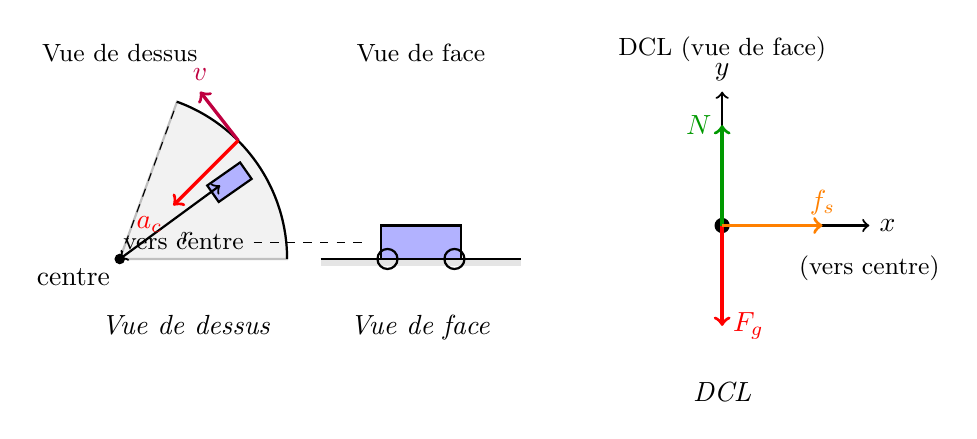
\begin{tikzpicture}[scale=0.85]
    % Vue de dessus (gauche)
    \begin{scope}[xshift=-4.5cm]
        \node[above] at (0,2.8) {\small Vue de dessus};
        
        % Virage (arc de cercle)
        \draw[thick, gray!50, fill=gray!10] (0,0) -- (2.5,0) arc (0:70:2.5) -- cycle;
        \draw[thick] (2.5,0) arc (0:70:2.5);
        \draw[dashed] (0,0) -- (0.86,2.35);
        
        % Voiture (rectangle)
        \begin{scope}[rotate=35, shift={(2,0)}]
            \draw[thick, fill=blue!30] (-0.3,-0.15) rectangle (0.3,0.15);
        \end{scope}
        
        % Centre et rayon
        \filldraw[black] (0,0) circle (2pt) node[below left] {centre};
        \draw[<->, thick] (0,0) -- (1.5,1.1) node[midway, below right] {$r$};
        
        % Vitesse tangentielle
        \draw[->, very thick, purple] (1.77,1.77) -- (1.2,2.5) node[above] {$\vect{v}$};
        
        % Accélération centripète
        \draw[->, very thick, red] (1.77,1.77) -- (0.8,0.8) node[below left] {$\vect{a}_c$};
        
        \node[below] at (1,-0.7) {\textit{Vue de dessus}};
    \end{scope}
    
    % Vue de face (milieu)
    \begin{scope}[xshift=0cm]
        \node[above] at (0,2.8) {\small Vue de face};
        
        % Route
        \fill[gray!20] (-1.5,-0.1) rectangle (1.5,0);
        \draw[thick] (-1.5,0) -- (1.5,0);
        
        % Voiture
        \draw[thick, fill=blue!30] (-0.6,0) rectangle (0.6,0.5);
        \draw[thick] (-0.5,0) circle (0.15);
        \draw[thick] (0.5,0) circle (0.15);
        
        % Centre du virage
        \draw[dashed] (-2.5,0.25) -- (-0.8,0.25);
        \node[left] at (-2.5,0.25) {\small vers centre};
        
        \node[below] at (0,-0.7) {\textit{Vue de face}};
    \end{scope}
    
    % DCL (droite) - vue de face
    \begin{scope}[xshift=4.5cm]
        \node[above] at (0,2.8) {\small DCL (vue de face)};
        
        % Point
        \filldraw[black] (0,0.5) circle (3pt);
        
        % Axes
        \draw[->, thick] (0,0.5) -- (2.2,0.5) node[right] {$x$};
        \draw[->, thick] (0,0.5) -- (0,2.5) node[above] {$y$};
        \node[below] at (2.2,0.2) {\small (vers centre)};
        
        % Forces
        \draw[->, very thick, red] (0,0.5) -- (0,-1) node[right] {$\vect{F}_g$};
        \draw[->, very thick, green!60!black] (0,0.5) -- (0,2) node[left] {$\vect{N}$};
        \draw[->, very thick, orange] (0,0.5) -- (1.5,0.5) node[above] {$\vect{f}_s$};
        
        \node[below] at (0,-1.7) {\textit{DCL}};
    \end{scope}
\end{tikzpicture}
\end{center}

Forces sur la voiture :
\begin{itemize}
    \item Poids : $F_g = mg$ (vers le bas)
    \item Normale : $N$ (vers le haut)
    \item Frottement statique : $f_s$ (horizontal, vers le centre du virage)
\end{itemize}

C'est le frottement qui fournit la force centripète nécessaire au virage.

\textbf{\underline{Étape 2 — AXES}}

$x$ : horizontal, vers le centre du virage (direction radiale)

$y$ : vertical, vers le haut

\textbf{\underline{Étape 3 — ÉQUATIONS DE NEWTON}}

Selon $y$ (pas d'accélération verticale) :
\begin{equation}
    N - mg = 0 \implies N = mg \tag{1}
\end{equation}

Selon $x$ (accélération centripète $a_c = v^2/r$) :
\begin{equation}
    f_s = ma_c = m\frac{v^2}{r} \tag{2}
\end{equation}

Pour que la voiture ne dérape pas, le frottement doit rester dans les limites du frottement statique :
\begin{equation}
    f_s \leq \mu_s N = \mu_s mg \tag{3}
\end{equation}

\textbf{\underline{Étape 4 — ALGÈBRE}}

\textbf{a) Vitesse maximale :}

À la limite du dérapage, $f_s = \mu_s N$. En combinant (2) et (3) :
\[ m\frac{v_{\max}^2}{r} = \mu_s mg \]
\[ v_{\max}^2 = \mu_s g r \]
\[ v_{\max} = \sqrt{\mu_s g r} = \sqrt{0{,}7 \times 9{,}81 \times 60} \]
\[ v_{\max} = \sqrt{412} = 20{,}3~\text{m/s} \]
\[ \boxed{v_{\max} = 73{,}1~\text{km/h}} \]

\textbf{b) À 80 km/h :}

$v = 80~\text{km/h} = 22{,}2~\text{m/s}$

Force centripète nécessaire :
\[ F_c = m\frac{v^2}{r} = 1400 \times \frac{22{,}2^2}{60} = 1400 \times 8{,}21 = 11\,500~\text{N} \]

Force de frottement maximale disponible :
\[ f_{s,\max} = \mu_s mg = 0{,}7 \times 1400 \times 9{,}81 = 9\,614~\text{N} \]

Comme $F_c = 11\,500~\text{N} > f_{s,\max} = 9\,614~\text{N}$ :

\[ \boxed{\text{Oui, la voiture va déraper!}} \]

\textbf{Vérification :} La vitesse maximale (73 km/h) est inférieure à 80 km/h, ce qui confirme le dérapage. Remarquons aussi que $v_{\max} = \sqrt{\mu_s g r}$ ne dépend pas de la masse : une voiture légère et un camion lourd ont la même vitesse maximale dans ce virage (si leurs pneus ont le même $\mu_s$).

\end{exemple}

\begin{pratiqueautonome}[title=Pratique autonome 2.9 — Navire en virage]
Un navire de 8\,000 tonnes effectue un virage circulaire de rayon 500~m à une vitesse de 15 nœuds (7{,}72~m/s).

\begin{enumerate}
    \item Quelle force centripète est nécessaire pour ce virage?
    \item Cette force est fournie par la résistance latérale de l'eau sur la coque. Si le navire accélère à 20 nœuds dans le même virage, de quel facteur la force centripète augmente-t-elle?
    \item À 20 nœuds, la cargaison sur le pont subit une accélération. Quel coefficient de frottement statique minimal est nécessaire pour qu'une caisse ne glisse pas?
\end{enumerate}

\vspace{4cm}

\tcblower
\textit{Réponses :} 1) $F_c = 952$~kN \quad 2) Facteur 1{,}78 (car $F_c \propto v^2$) \quad 3) $\mu_s = 0{,}021$
\end{pratiqueautonome}
